\documentclass[final]{beamer}

\usepackage[orientation=landscape,size=a0,scale=1.2]{beamerposter} 

\usepackage[utf8]{inputenc}
\usepackage[T1]{fontenc}
\usepackage{graphicx}
\usepackage{booktabs}
\usepackage{amsmath,amssymb}
\usepackage{colortbl}
\usepackage{multicol}
\usepackage{braket}

\definecolor{cvprblue}{RGB}{0, 115, 188}
\setbeamercolor{headline}{bg=white,fg=black}
\setbeamercolor{block title}{bg=cvprblue,fg=white}
\setbeamercolor{block body}{bg=white,fg=black}
\setbeamercolor{structure}{fg=cvprblue}

\setbeamertemplate{navigation symbols}{}
\setbeamertemplate{block begin}{
    \vskip2ex
    \begin{beamercolorbox}[ht=3.5ex,dp=1.5ex,center,rounded=false,shadow=false]{block title}
        \usebeamerfont*{block title}\insertblocktitle
    \end{beamercolorbox}
    {\ifbeamercolorempty[bg]{block body}{}{\nointerlineskip\vskip-0.5pt}}
    \usebeamerfont{block body}
    \begin{beamercolorbox}[sep=1ex,vmode]{block body}
    \ifbeamercolorempty[bg]{block body}{\vskip-2.5ex}{\vskip-0.5ex}
}

\usepackage[most]{tcolorbox}
\newtcbox{\highlight}[1][cvprblue]{        
    on line, 
    arc=3pt,                              
    colback=#1!25,                         
    colframe=#1!60,                        
    before upper=\strut, 
    boxrule=0pt,                          
    boxsep=0pt, 
    left=4pt, right=4pt, top=2pt, bottom=2pt
}
\setbeamertemplate{block end}{\end{beamercolorbox}\vskip1.5ex}

\begin{document}
\begin{frame}[t]

% logo - title - logo
\begin{beamercolorbox}[wd=\textwidth, sep=2cm]{headline}
    \begin{columns}[c]
        \column{.15\textwidth}
            \centering
            
\includegraphics[height=8cm]{figure/UAH_Primary_2025UPDATE_RGB_03.png} 
        
        \column{.7\textwidth}
            \centering
            \vspace{1cm}
            {\VeryHuge \textbf{\linespread{1.2}\selectfont The PID Controller Strikes Back: Classical Controller Helps Mitigate Barren Plateaus in Noisy Variational Quantum Circuits}} \\[1cm]
            {\huge Zhehao Yi$^1$, Rahul Bhadani$^1$} \\[0.5cm]
            {\Large $^1$AI, Autonomy, Resilience, Control Lab, Electrical \& Computer Engineering Department, University of Alabama in Huntsville} \\[0.5cm]
            {\texttt{\{zhehao.yi, rahul.bhadani\}@uah.edu}}
            \vspace{1cm}
            
        \column{.15\textwidth}
            \centering
            
\includegraphics[height=8cm]{figure/LogoWithText.pdf}
            
    \end{columns}

\end{beamercolorbox}
\rule{\textwidth}{2pt}

\begin{columns}[t]
    \hspace{0.5cm}
    \begin{column}{.23\textwidth}
        \begin{block}{\textbf{Introduction}}
            % \small
            \vspace{0.4cm}
            Variational quantum algorithms (VQAs) combine the advantages of classical optimization and quantum computation. However, when optimized using gradient descent, VQAs often suffer from the vanishing gradient problem, commonly known as the barren plateau. In this work, we propose a hybrid approach that integrates a classical proportional-integral-derivative (PID) controller with a neural network to update the parameters of variational quantum circuits, which aims to mitigate the barren plateau. The proposed algorithm is tested on randomly generated quantum input states and random quantum circuits with parametric noise to evaluate its universality.
        \begin{beamercolorbox}[wd=\linewidth, sep=1ex, rounded=true]{block body}
            \centering
            \begin{minipage}{0.3\linewidth}
                \centering
                
\includegraphics[width=0.7\linewidth]{figure/code.pdf} \\
                \scriptsize \textbf{Code (GitHub)}
            \end{minipage}
            \hfill
            \begin{minipage}{0.3\linewidth}
                \centering
                
\includegraphics[width=0.7\linewidth]{figure/paper.pdf} \\
                \scriptsize \textbf{Paper (L4DC)}
            \end{minipage}
            \hfill
            \begin{minipage}{0.3\linewidth}
                \centering
                
\includegraphics[width=0.7\linewidth]{figure/lab.pdf} \\
                \scriptsize \textbf{AARC Lab}
            \end{minipage}
        \end{beamercolorbox}
        \end{block}

        \begin{block}{\textbf{Background}}
            \begin{itemize}
                \item \textbf{Motivation:} Promise of VQAs in NISQ era and Inspiration from Classical Control.
                \item \textbf{Challenge:} The Barren Plateau (BP) Problem, Hardware \& Parametric Noise and Non-linearity vs. Linearity.
            \end{itemize}
            \centering
            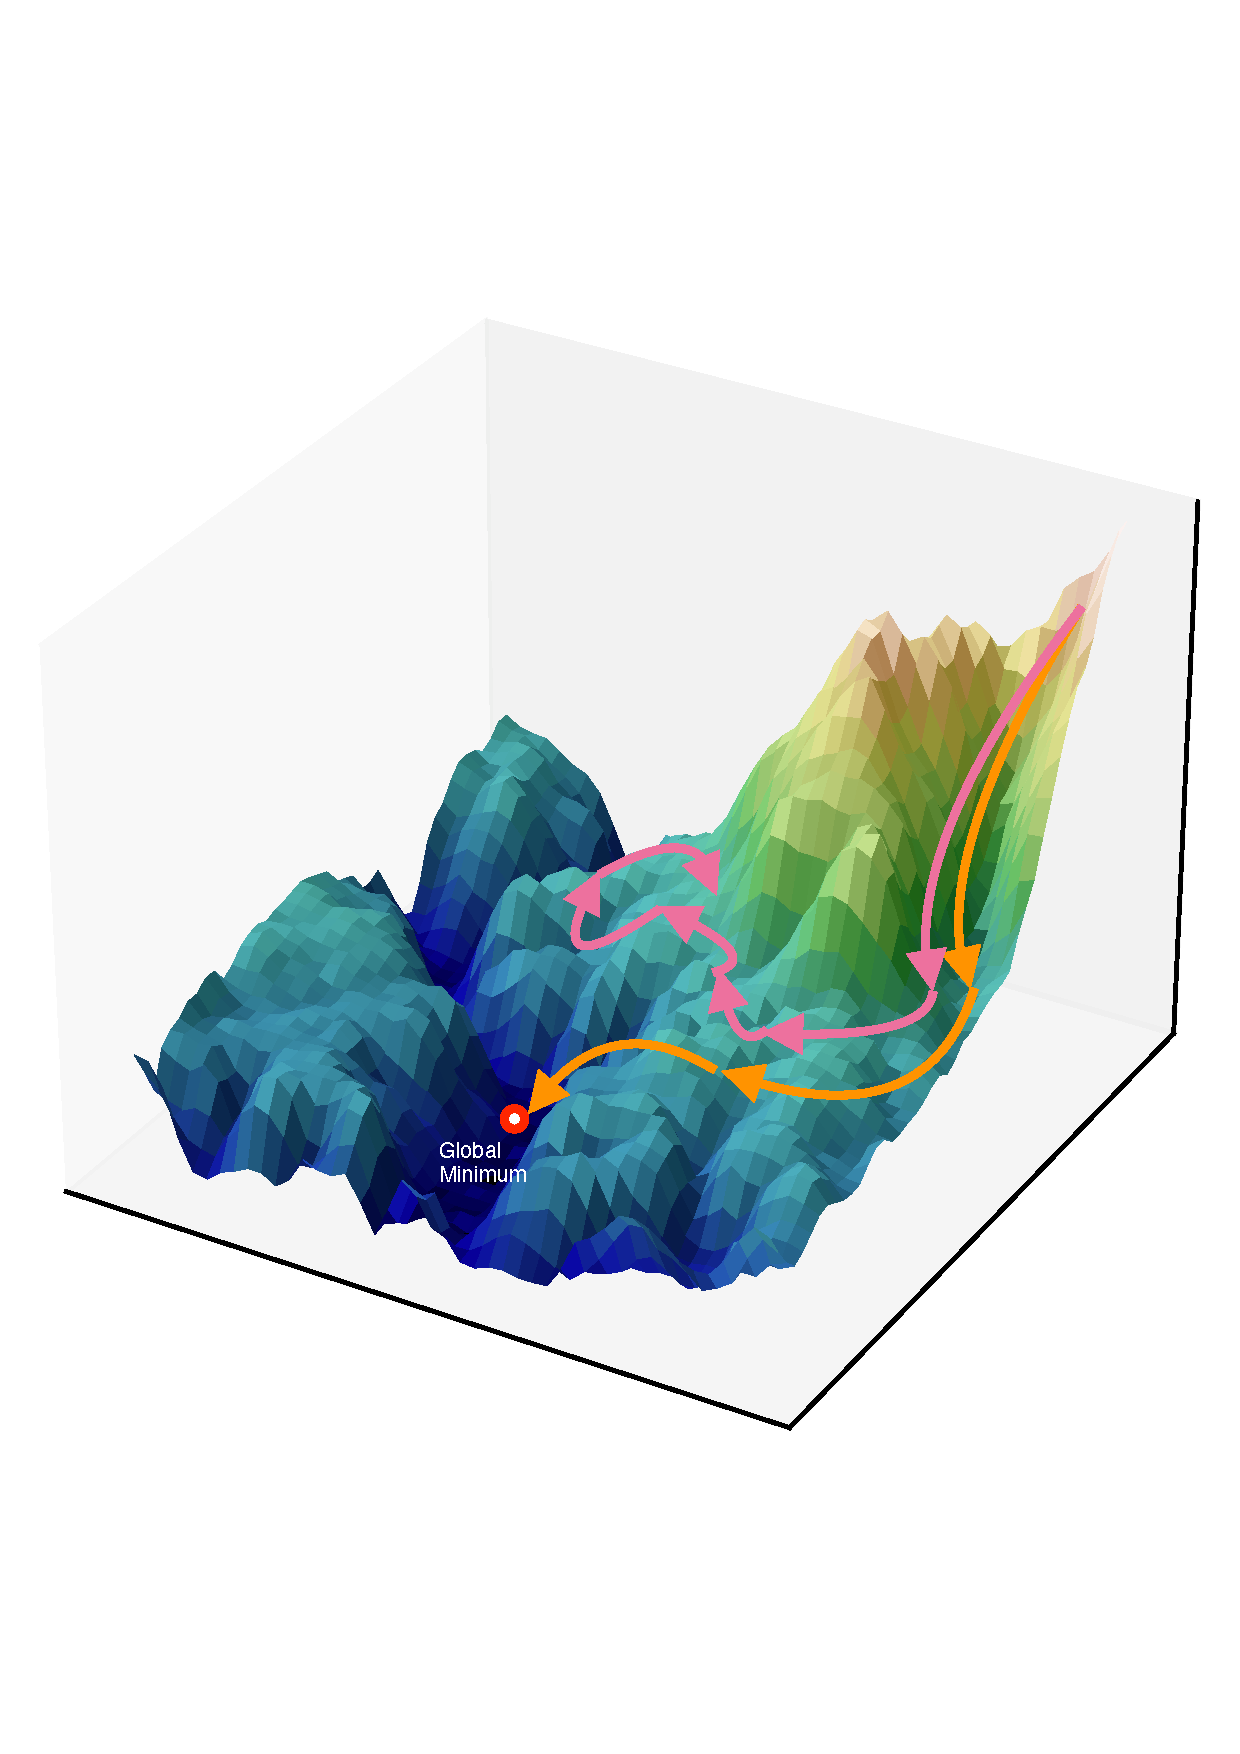
\includegraphics[width=0.9\linewidth]{figure/bp.pdf}
            \captionof{Figure 1:}{ Example of the Barren Plateau phenomenon in VQAs. The orange line represents the training trajectory overcome the barren plateau to reach the global minimum, while the pink line represents the training trajectory stuck in the barren plateau.}
        \end{block}
    \end{column}


\begin{column}{.48\textwidth}
    \begin{block}{\textbf{Quantum Setup}}
        \vspace{0.4cm}
        \begin{columns}[c]
            \column{.45\textwidth}
                \textbf{\large A. Random Input States} \\
                \small
                To evaluate the universality of the NPID, we use the random quantum $\ket{\psi}$ state as input:
                \begin{equation*}
                    \ket{\psi_{in}} = \bigotimes_1^{n}\{R_z(\theta_k)R_y(\theta_j)R_x(\theta_i)\ket{0}\}
                \end{equation*}
                The parameters $\theta_i, \theta_j, \theta_k$ are randomly sampled from a uniform distribution over $[0, 2\pi]$.

                \vspace{0.5cm}
                \textbf{\large B. Random Quantum Circuit} \\
                The variational circuit $\mathcal{U}(\theta)$ consists of $L$ layers of parametric rotations and entanglers

                \vspace{0.5cm}
                \textbf{\large C. Cost Function} \\
                \begin{equation*}
                    \mathcal{L} = 1- \frac{1}{n}\sum_{i1}^{n}Tr\{ ( \ket{0}\bra{0}_i \otimes I_{\hat{i}} ) \ket{\psi_{in}} \}
                \end{equation*}

            \column{.5\textwidth}
                \centering
                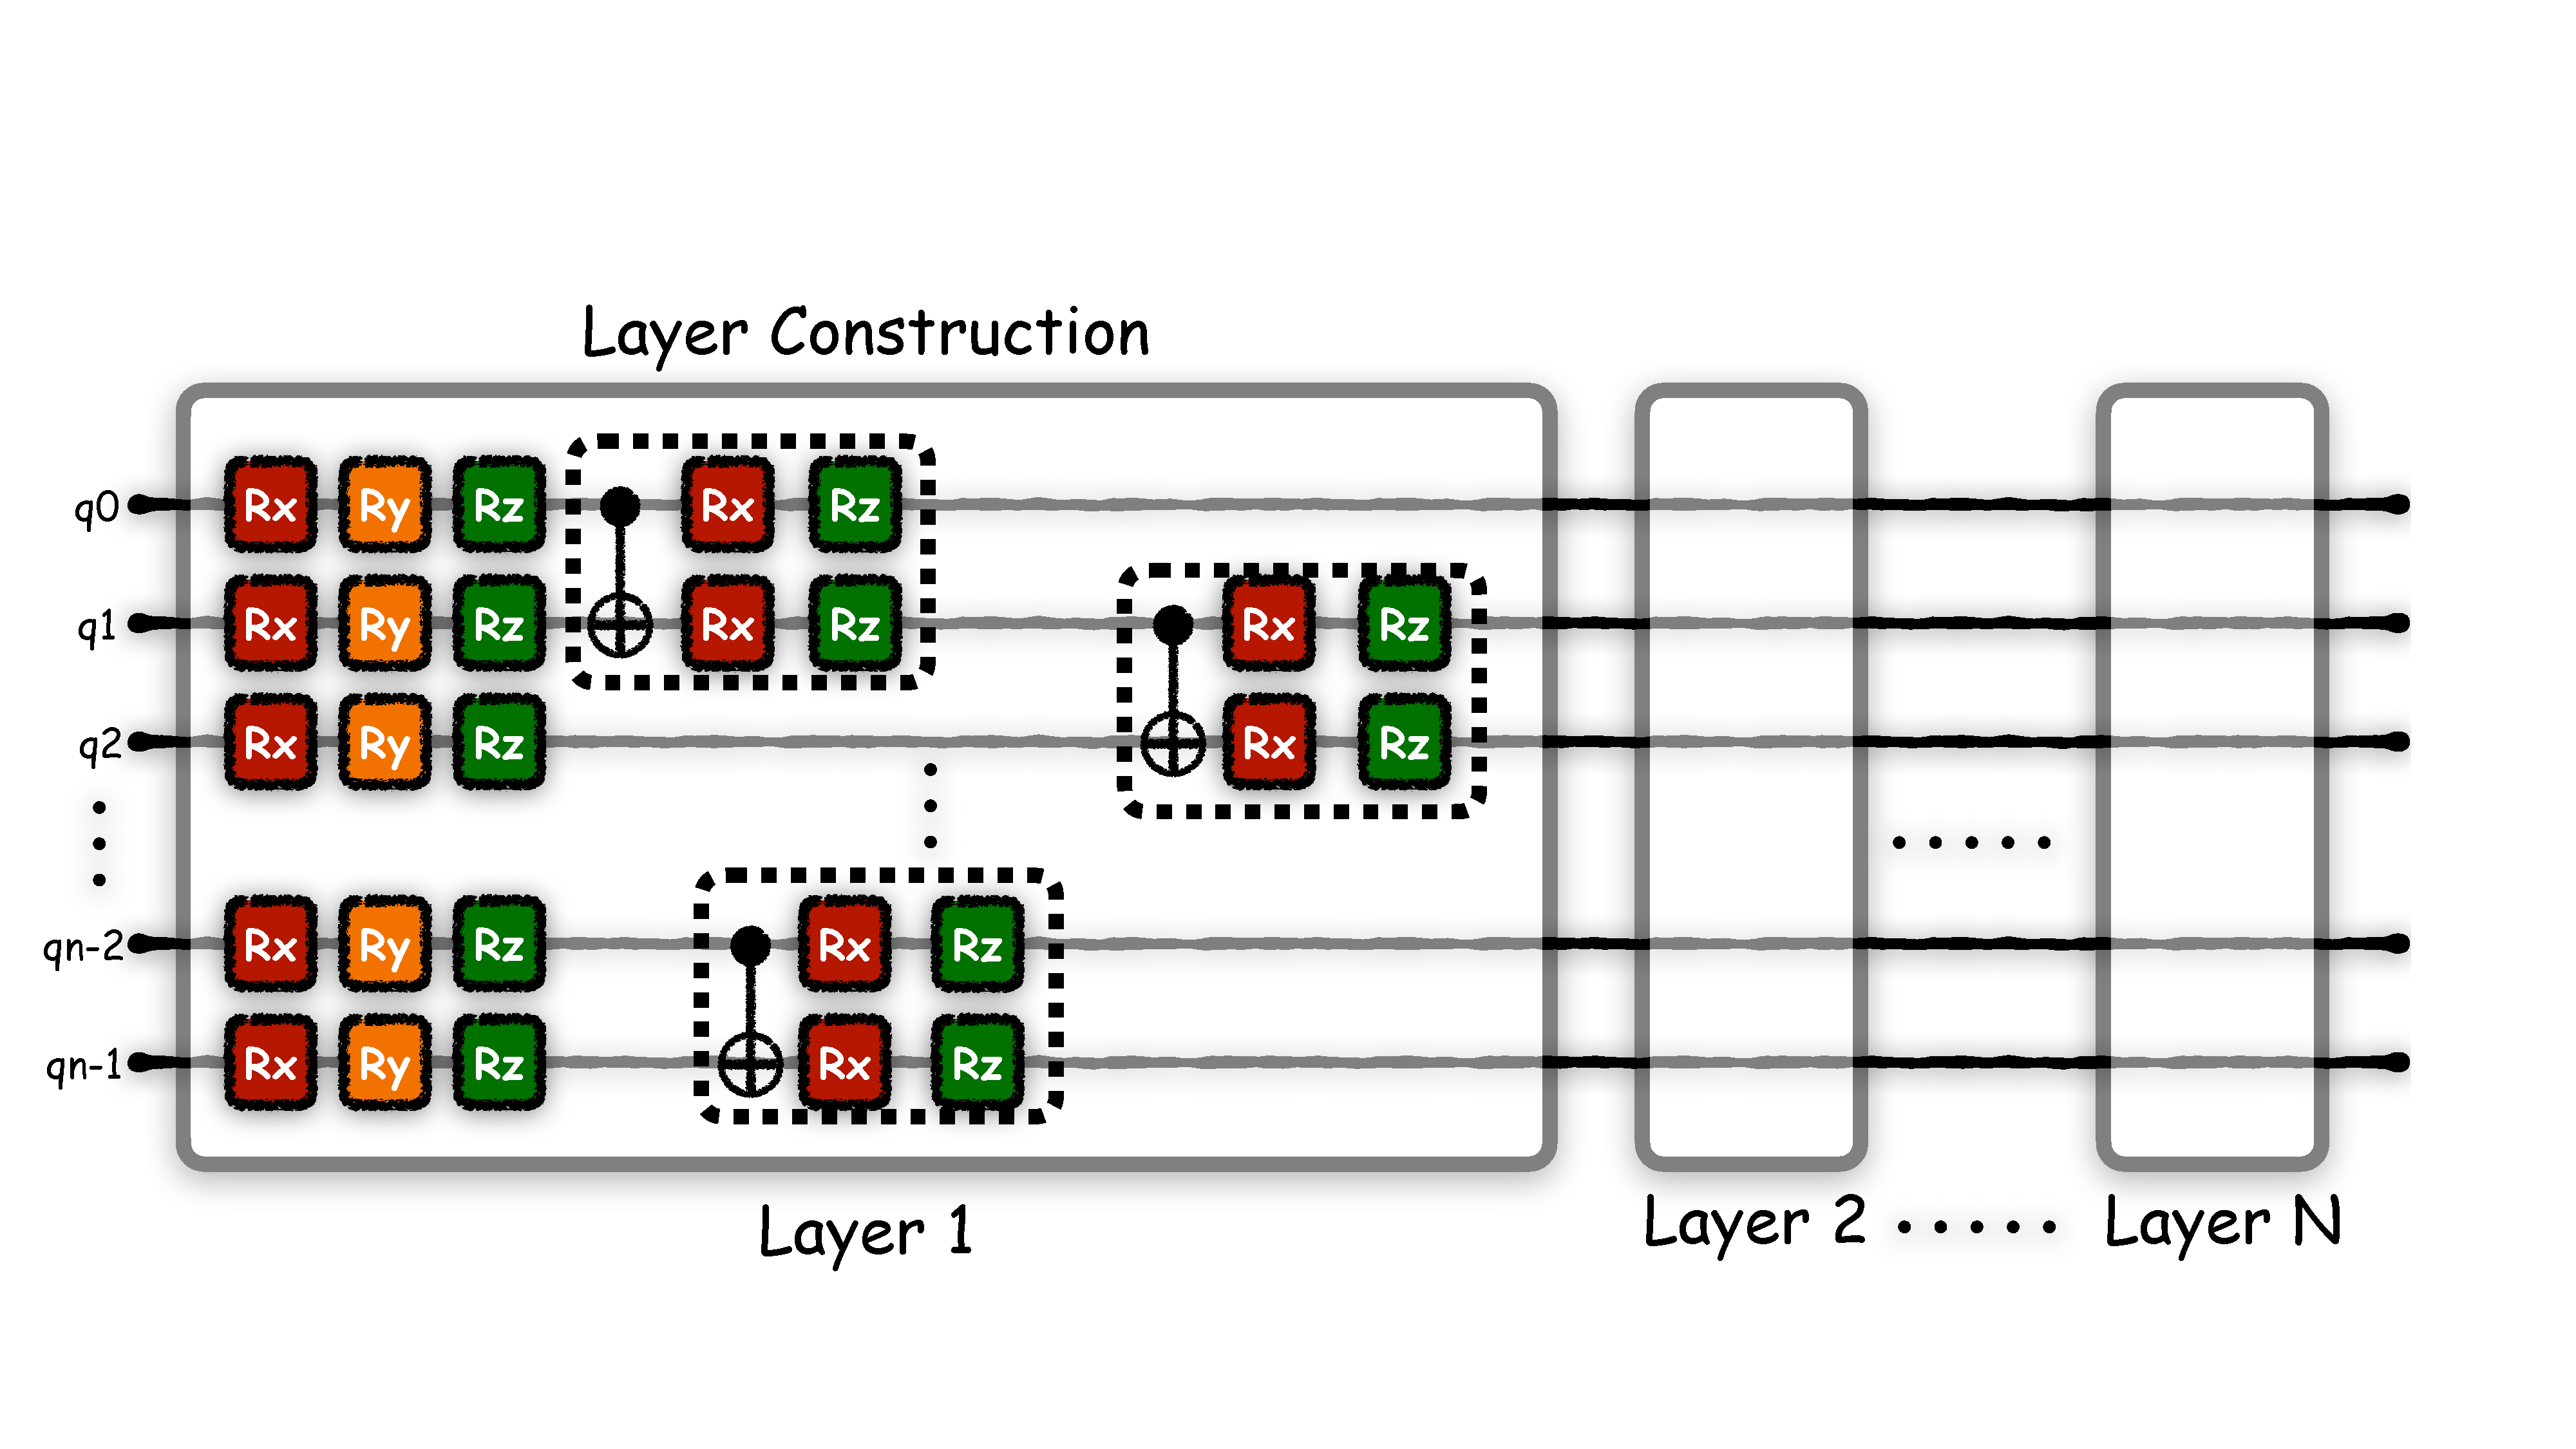
\includegraphics[width=1\linewidth]{figure/randomquantumcircuit.pdf} 
                \captionof{Figure 2: }{The Construction of the random quantum circuit. The gray boxes represent individual circuit layers, while the black dashed boxes indicate the gates applied between pairs of randomly selected qubits.}
        \end{columns}
    \end{block}
    \begin{block}{\textbf{Neural PID (NPID) Framework}}
        \centering
        \vspace{1cm}
        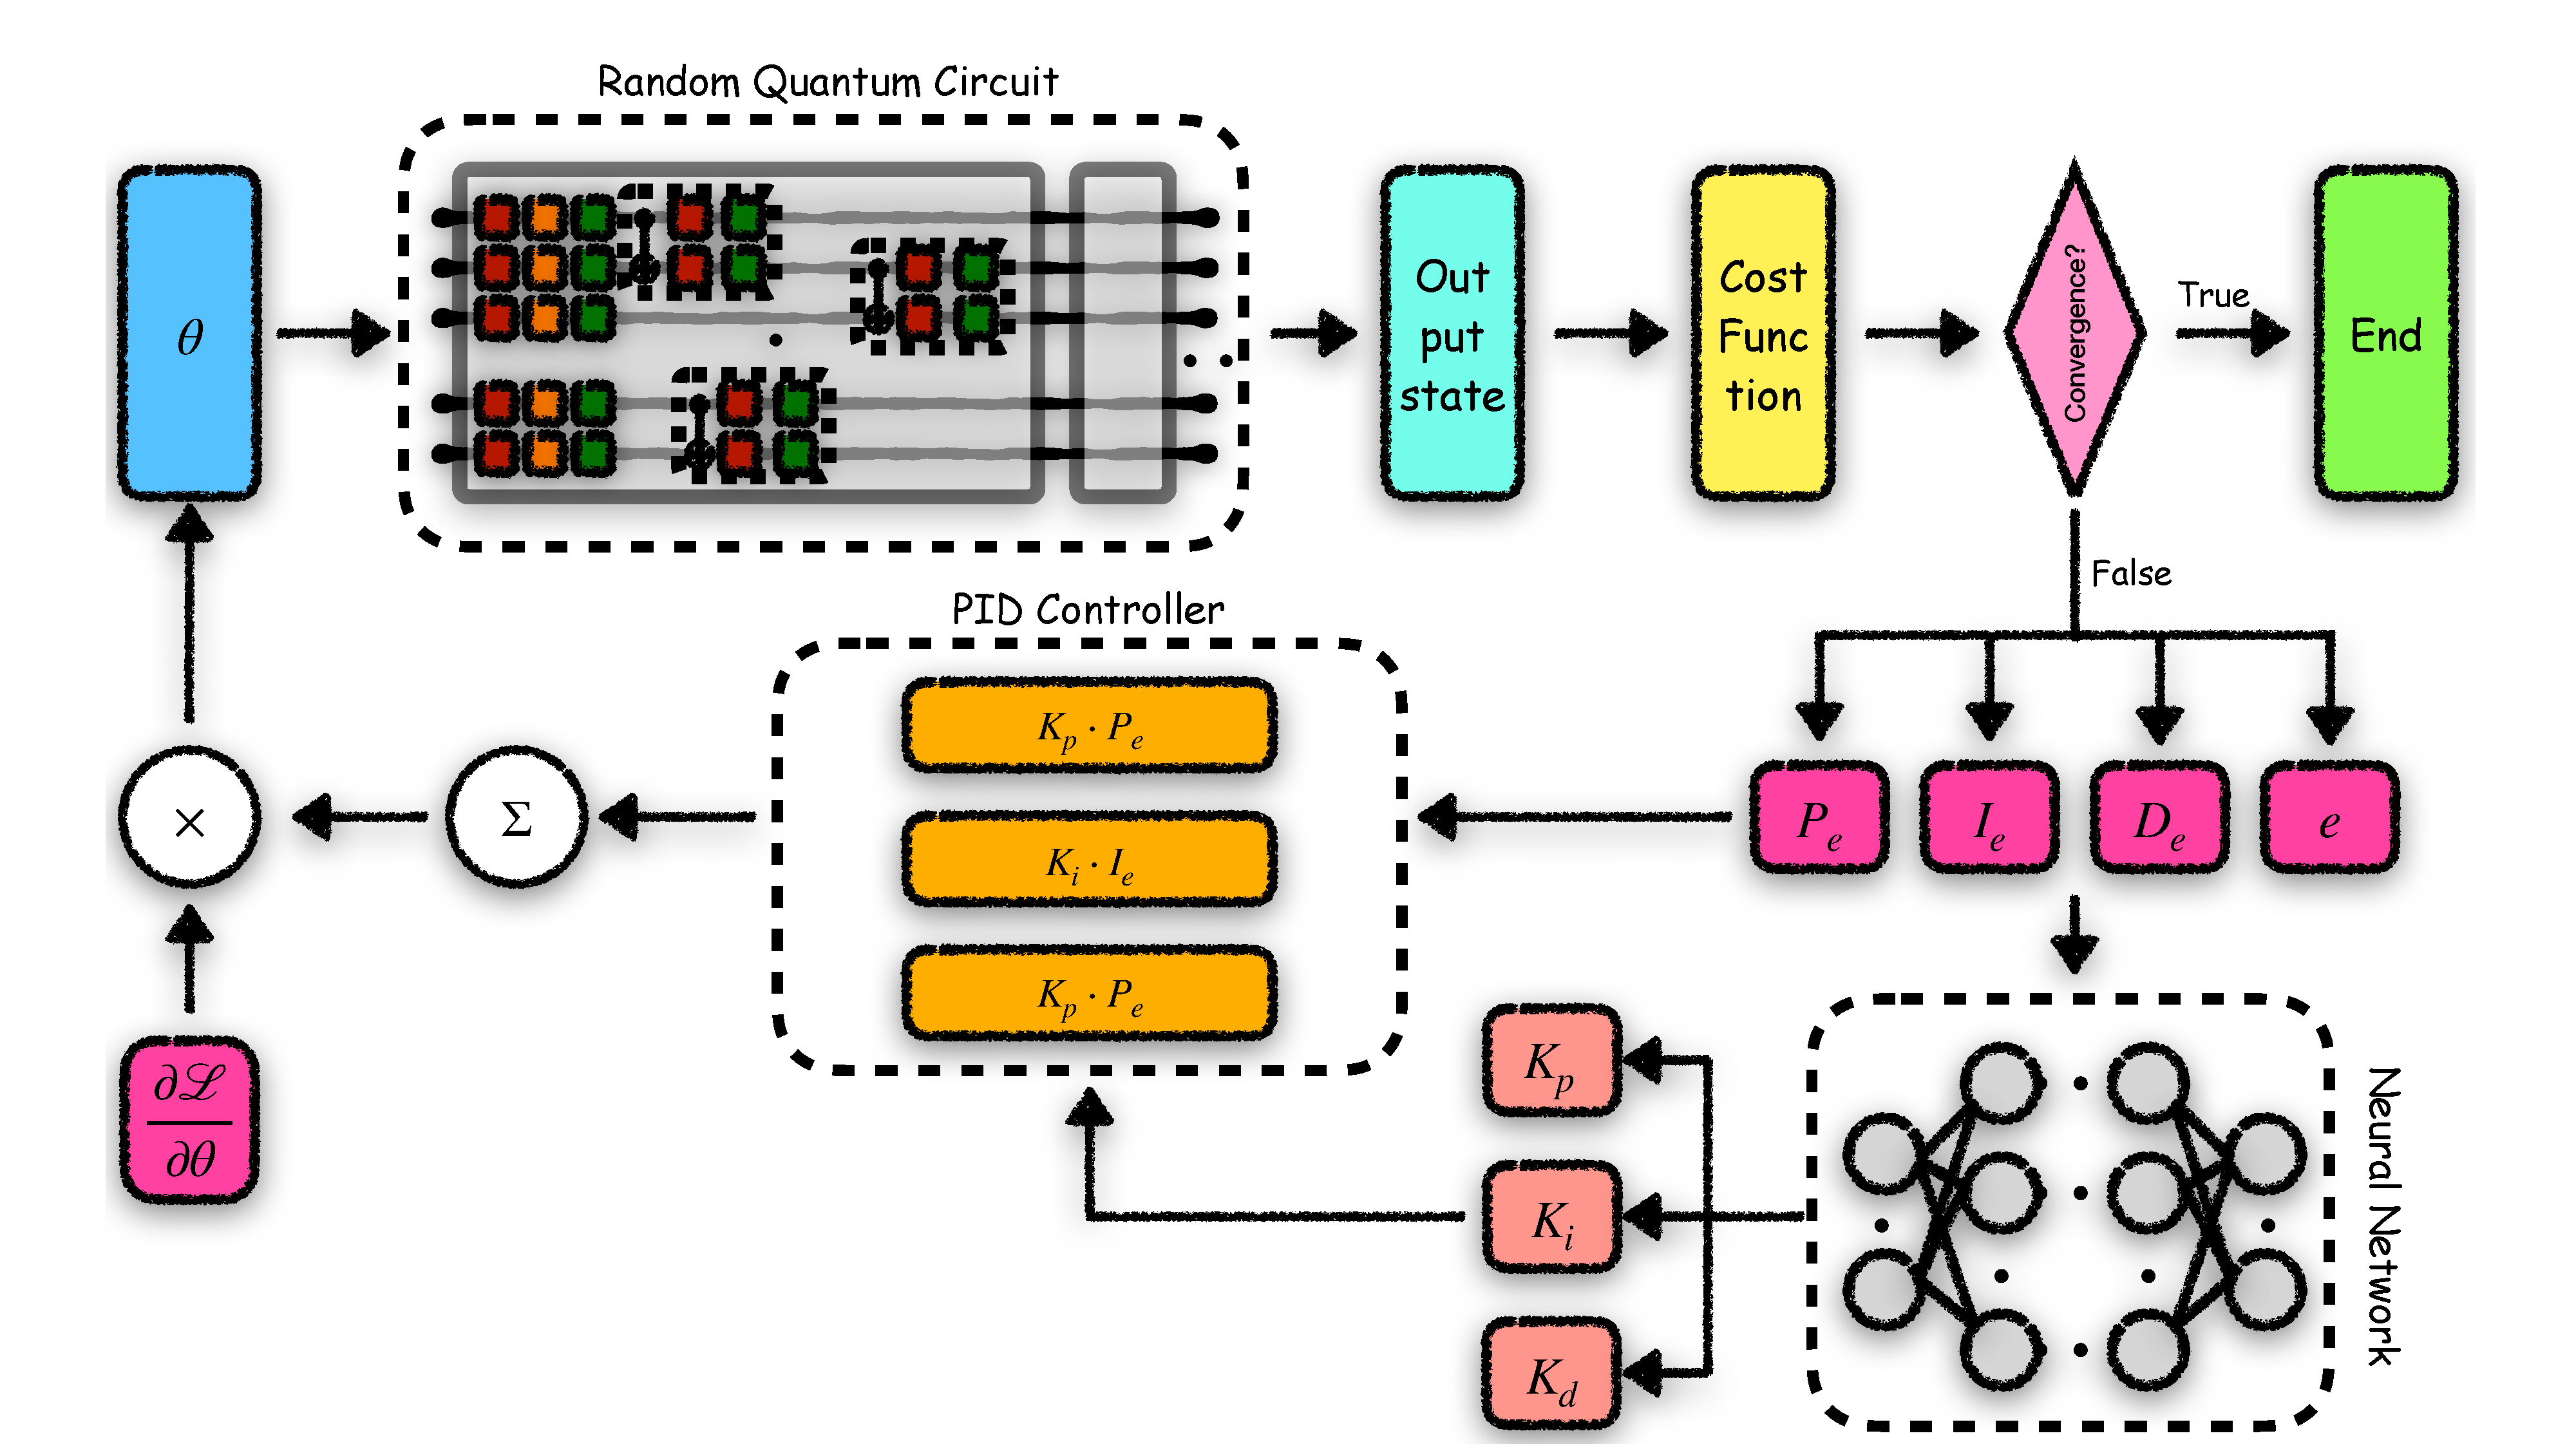
\includegraphics[width=0.7\linewidth]{figure/NPID.pdf} \\
        \captionof{Figure 3:}{ In NPID, the computed loss value $e$ serves two purposes: it is used in the PID control computation to update the parameter list $\theta$ of the quantum circuit, and simultaneously drives the gradient updates of the neural network that generates the PID gains.}
        
        \vspace{1cm}
        \begin{beamercolorbox}[wd=0.98\linewidth, sep=1.5ex, rounded=true]{block body}
            \textbf{\large Algorithm: Circuit Parameter Update with NPID} \\
            \vspace{0.5cm}
            \begin{columns}[t]
                \column{.45\textwidth}
                    \textbf{Step 1: Error Processing}
                    \begin{itemize}
                        \item Proportional: $P_e = e$
                        \item Integral: $I_e = e + e_{pre}$
                        \item Derivative: $D_e = e - e_{pre}$
                    \end{itemize}
                    \textbf{Step 2: Dynamic Gain Tuning}
                    \begin{equation*}
                        [K_p, K_i, K_d] = \phi(e, P_e, I_e, D_e)
                    \end{equation*}

                \column{.5\textwidth}
                    \textbf{Step 3: PID Control Signal}
                    \begin{equation*}
                        O_{pid} = K_p P_e + K_i I_e + K_d D_e
                    \end{equation*}
                    \textbf{Step 4: Gradient Modulation}
                    \begin{equation*}
                        \hat{\theta}_{i+1} = \hat{\theta}_i - \eta \cdot \frac{\partial \mathcal{L}}{\partial \theta} \cdot O_{pid}
                    \end{equation*}
                    \small{\textit{*where $\eta$ is the learning rate.}}
            \end{columns}
        \end{beamercolorbox}
    \end{block}
\end{column}

    \begin{column}{.23\textwidth}

    \begin{block}{\textbf{Simulations Performance Analysis}}
        \centering
        \vspace{0.4cm}
        
        \begin{minipage}{0.48\linewidth}
            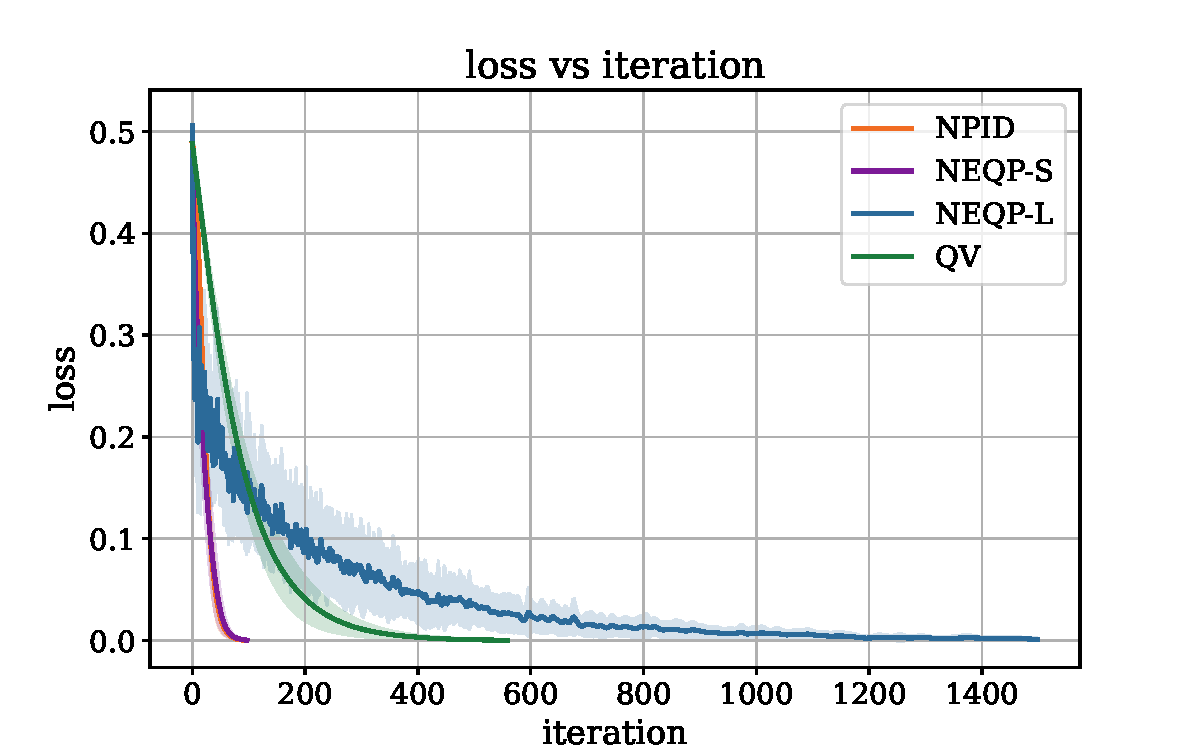
\includegraphics[width=\linewidth]{figure/loss_iter_7.pdf}
        \end{minipage}
        \hfill
        \begin{minipage}{0.48\linewidth}
            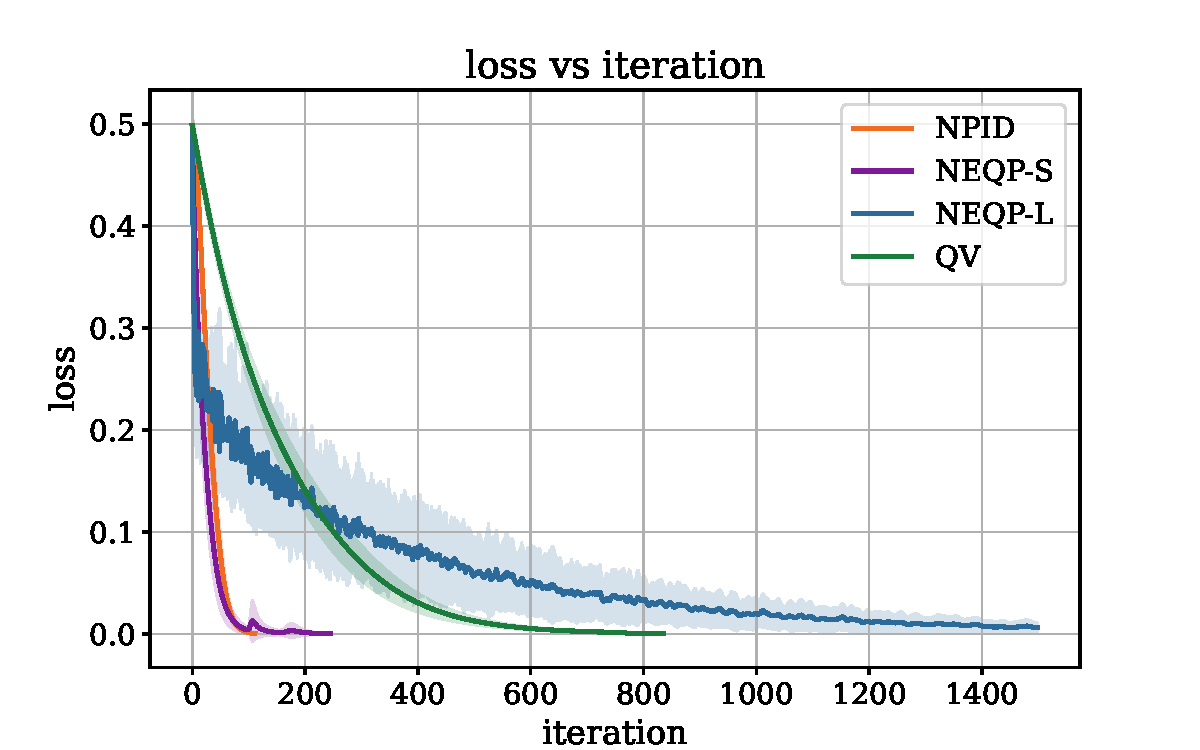
\includegraphics[width=\linewidth]{figure/loss_iter_8.pdf}
        \end{minipage}
        
        \vspace{0.2cm}
        
       
        \begin{minipage}{0.48\linewidth}
            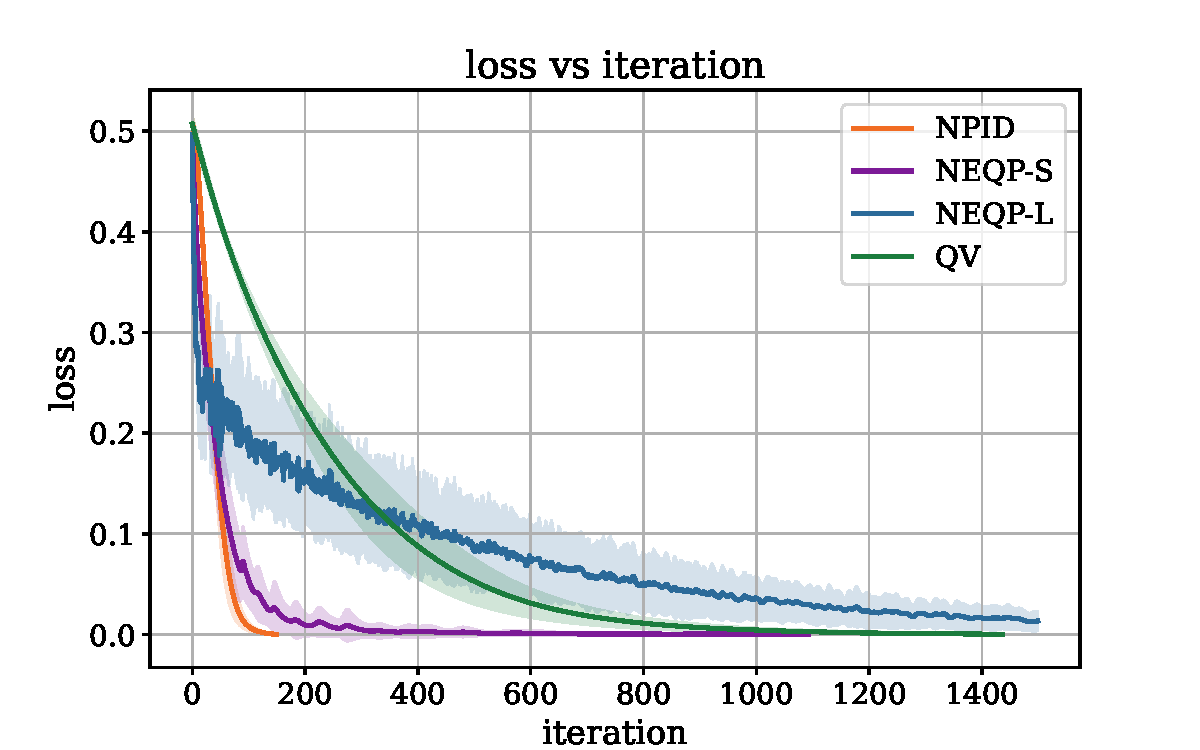
\includegraphics[width=\linewidth]{figure/loss_iter_9.pdf}
        \end{minipage}
        \hfill
        \begin{minipage}{0.48\linewidth}
            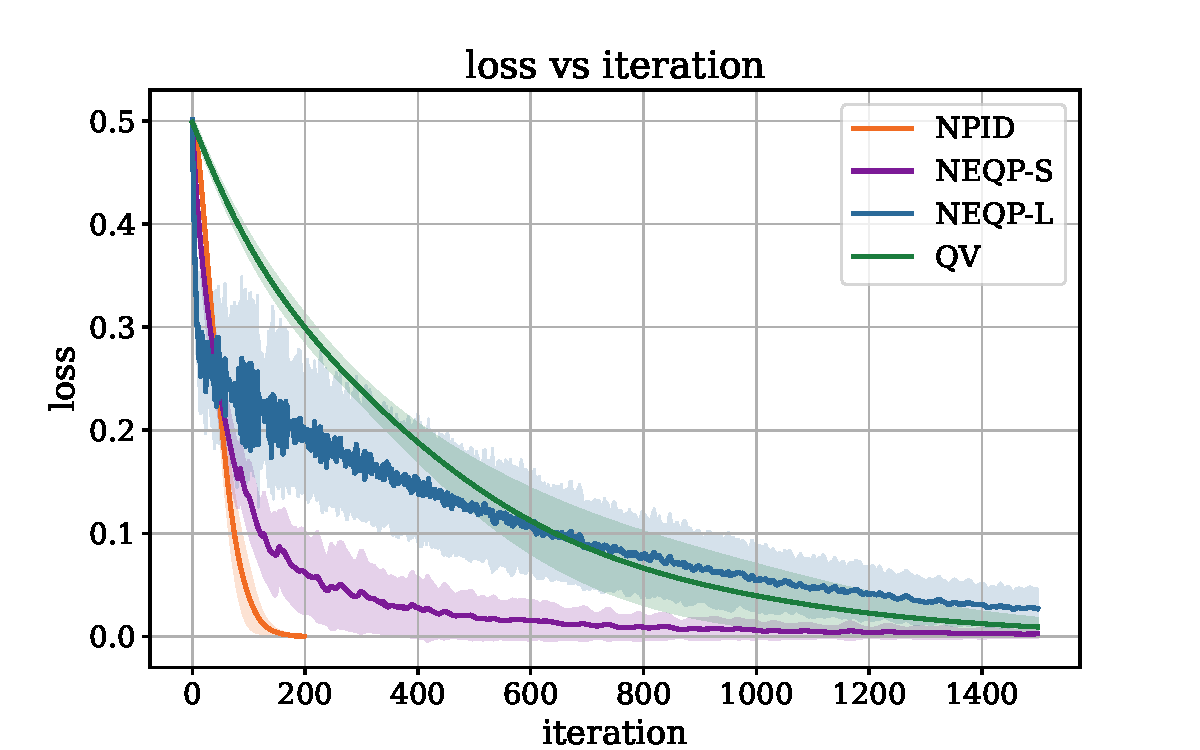
\includegraphics[width=\linewidth]{figure/loss_iter_10.pdf}
        \end{minipage}

        \vspace{0.2cm}
        
        
        \begin{minipage}{0.48\linewidth}
            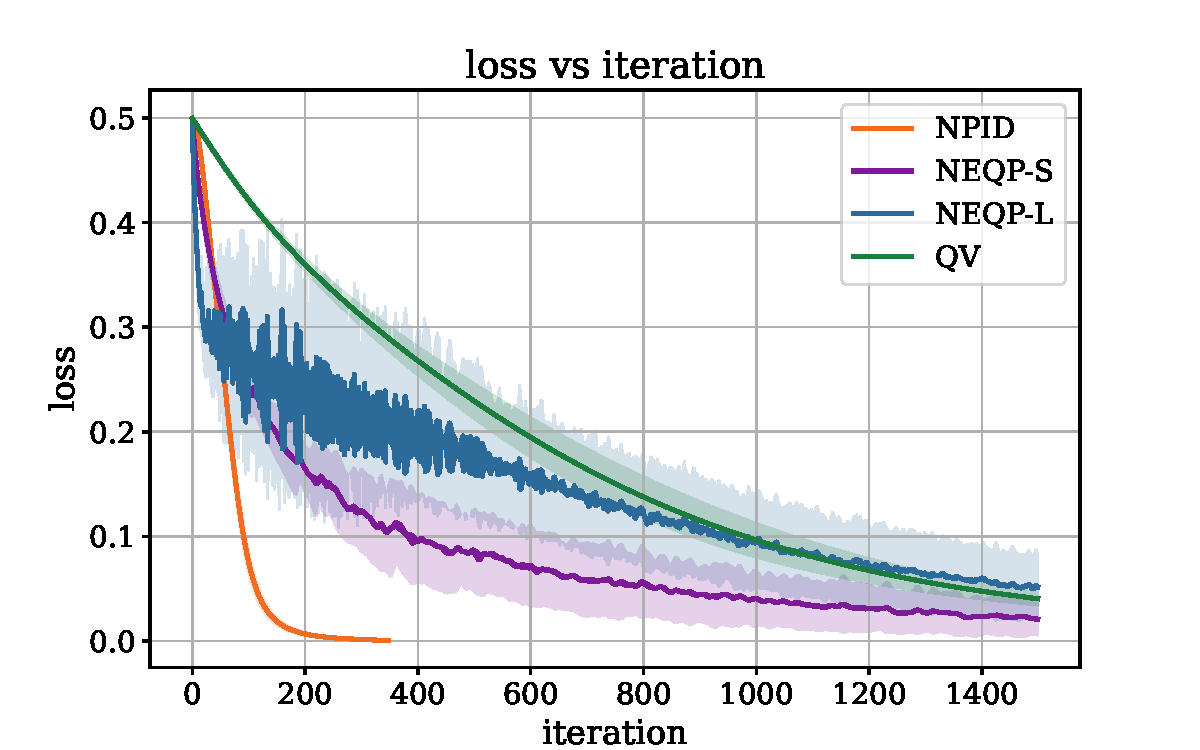
\includegraphics[width=\linewidth]{figure/loss_iter_11.pdf}
        \end{minipage}
        \hfill
        \begin{minipage}{0.48\linewidth}
            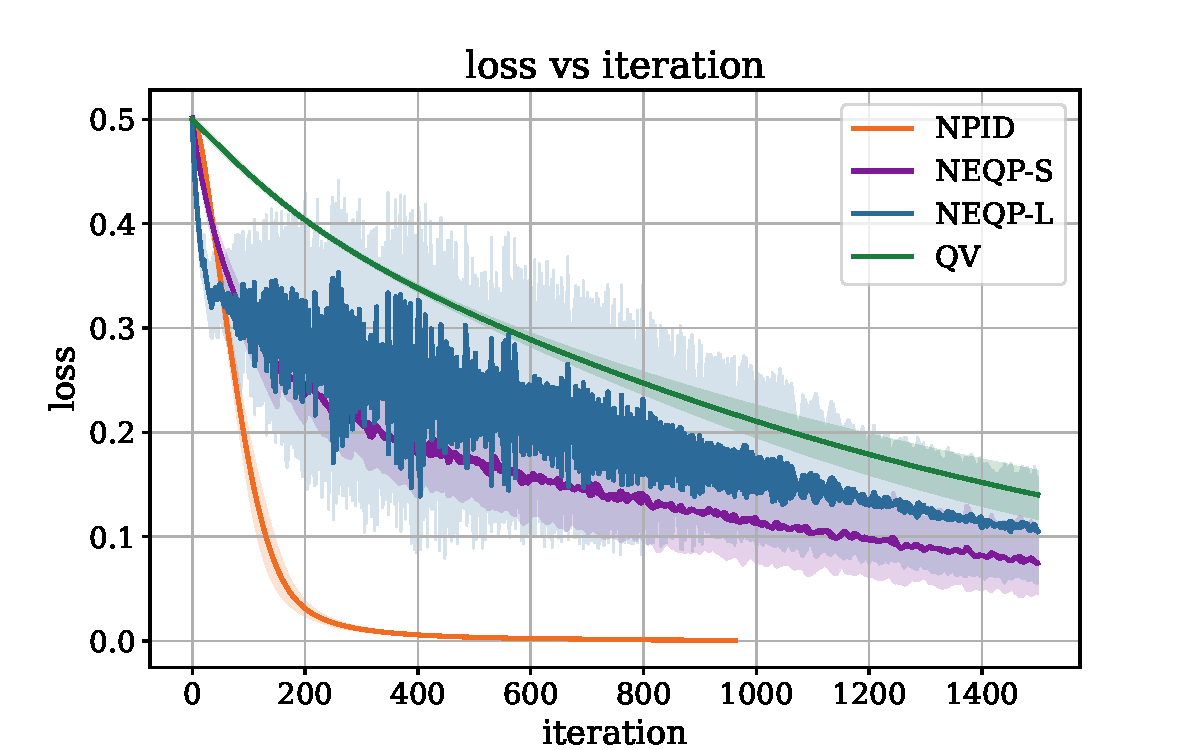
\includegraphics[width=\linewidth]{figure/loss_iter_12.pdf}
        \end{minipage}
        
        \captionof{Figure 4: }{Convergence speed comparison across 6 different number of qubits (Form 7 to 12). NPID consistently achieves the target loss faster than NEQP and QV baselines.}

        \rule{\textwidth}{2pt}
        \textbf{\Average Iterations with Different Parametric Noise} \\
        \vspace{0.3cm}
        \scriptsize
        \renewcommand{\arraystretch}{1.2}
        \begin{tabular}{ccccccc}
        \hline
        \textbf{Noise Rate} & \textbf{7 Qubits} & \textbf{8 Qubits} & \textbf{9 Qubits} & \textbf{10 Qubits} & \textbf{11 Qubits} &\textbf{12 Qubits} \\ 
        \hline
        0.03 & 74 & 90 & 127 & 171 & 304 & 845 \\ 
        0.05  & 90 & 94 & 147 & 161 & 285 & 858 \\ 
        0.07  & 79 & 92 & 133 & 156 & 304 & 911 \\ 
        0.09 & 83 & 89 &  143 & 172 & 281 &  817 \\
        \hline
        \textbf{Fluctuation Rate} & 7.18\% & 2.10\% & 5.76\% & 4.08\% & 3.61\% &  3.98\%\\
        \hline
        \end{tabular}
        
        \vspace{0.4cm}
        \footnotesize \textbf{Mean Fluctuation Rate: \highlight[cvprblue]{4.45\%}}
    \end{block}

   
    \begin{block}{\textbf{Conclusion}}
        \begin{itemize}
            \item \textbf{High Efficiency:} 2--9$\times$ faster convergence speed.
            \item \textbf{Barren Plateau Mitigation:} Successfully trains deep random circuits where classical optimizers fail.
            \item \textbf{Robustness:} Maintains stability ($<$5\% fluctuation) under NISQ noise.
        \end{itemize}
    \end{block}

    \begin{block}{\textbf{References}}
        \small
        1. M. Cerezo, et al. Cost function dependent barren plateaus in shallow parametrized quantum circuits. Nature Communications, 12(1):1791, 2021b. \\
        2. L. Friedrich and J. Maziero. Avoiding barren plateaus with classical deep neural networks. Physical Review A, 106(4):042433, 2022. \\
        3. Z. Yi, et al. Enhancing variational quantum circuit training: an improved neural network approach for barren plateau mitigation. Physica Scripta, 100(8):086004, 2025.
    \end{block}

\end{column}
    
    \hspace{0.5cm}
\end{columns}

\end{frame}
\end{document}